\documentclass{article}
\usepackage[utf8]{inputenc}
\usepackage[style=authoryear,backend=biber]{biblatex}
\addbibresource{References.bib}
\newcommand{\theHalgorithm}{\arabic{algorithm}}
\usepackage{microtype}
\usepackage{graphicx}
\usepackage{subfigure}
\usepackage{subcaption}
\usepackage{booktabs}
\usepackage{amsmath}
\usepackage{amsfonts}
\usepackage{amsthm}
\usepackage{physics}
\usepackage{fancyvrb}
\usepackage{listings}
\usepackage{xcolor}
\usepackage{caption}
\usepackage{xurl}
\usepackage[dvipsnames]{xcolor}
\usepackage{tcolorbox}

% Define a new tcolorbox environment for callouts
\newtcolorbox{callout}[1][]{colback=gray!5!white, colframe=gray!75!black, fonttitle=\bfseries, title=#1}
\usepackage{url}
\usepackage{hyperref}
\usepackage{accessibility}
\usepackage{Coursework}

\begin{document}
\cwtitle{COMP1680 - Clouds, Grids and Virtualisation Coursework Report}
\begin{cwauthorlist}
\cwauthor{Azhar Muhammed - 001364857}
\cwauthor{Word Count: 3,921}
\end{cwauthorlist}

\part{Parallel Processing using Cloud Computing}

In the evolving landscape of computational technologies, small consultancy firms are faced with critical decisions regarding their computational infrastructure. The choice between adopting cloud computing services or investing in an onsite High-Performance Computing (HPC) system can significantly influence operational efficiency, scalability, and financial outcomes. This report aims to evaluate these options for a small consultancy firm comprising $30$ consultants, each requiring approximately $1,400$ CPU hours monthly. The analysis will focus on the advantages and disadvantages of leading cloud service providers such as Amazon Web Services (AWS), Microsoft Azure, and Google Cloud Platform (GCP) when compared to an onsite HPC system for handling multicore workloads using batch processing. A comprehensive financial comparison will also be provided, culminating in a recommendation that aligns with the strategic objectives of the firm.

\section{Analysis of Cloud Providers vs. Onsite HPC for Multicore Workloads}

Cloud computing has revolutionized the approach to handling computational workloads by providing scalable resources and flexible pricing models. On the other hand, onsite HPC systems, while offering dedicated resources, require substantial upfront investments and incur ongoing maintenance expenses. Each approach has its unique strengths and limitations, which will be discussed in detail.

\subsection{Advantages of Cloud Computing}

Cloud computing offers several advantages for small consultancies compared to onsite HPC systems:

\begin{enumerate}
    \item \textbf{Scalability and Flexibility:} Cloud services enable dynamic scaling of computational resources to match varying workload demands. This elasticity is crucial for batch processing tasks that may experience fluctuations in computational needs \parencite{armbrust2010cloud}. Cloud platforms allow the firm to increase or decrease resources seamlessly without additional capital expenditure.

    \item \textbf{Cost Efficiency:} Cloud providers operate on a pay-as-you-go model, which eliminates the need for substantial upfront investment in HPC hardware. This allows operational costs to align with actual usage, promoting financial predictability and minimizing the risk of over-investment in underutilized resources \parencite{li2019decision}.

    \item \textbf{Maintenance and Operational Overhead:} By utilizing cloud services, the responsibility of hardware maintenance, software updates, and security patching falls on the cloud provider, reducing the internal burden on IT staff \parencite{marinescu2013cloud}.

    \item \textbf{Access to Advanced Technologies:} Cloud platforms are frequently updated with the latest hardware and software innovations. Small firms can access these advanced technologies without incurring additional costs, which helps maintain competitiveness in a rapidly evolving industry \parencite{dillon2010cloud}.
\end{enumerate}

\subsection{Disadvantages of Cloud Computing}

While cloud computing offers numerous benefits, there are also potential drawbacks to consider:

\begin{enumerate}
    \item \textbf{Data Security and Compliance:} Relying on third-party providers raises concerns regarding data sovereignty and regulatory compliance, especially for sensitive client data \parencite{hashem2015bigdata}.

    \item \textbf{Service Availability:} Cloud services can experience unexpected outages that are beyond an organization's direct control, potentially disrupting critical business operations and affecting service-level agreements \parencite{Ibrahim2024}. Despite provider redundancy measures, downtime incidents can still impact business continuity and customer trust.

    \item \textbf{Unexpected Costs:} While cloud services offer financial flexibility, poor management of resources can lead to unexpectedly high expenses, such as data egress fees or underutilized instances \parencite{rehman2018cloud}.
\end{enumerate}

\subsection{Onsite HPC: Pros and Cons}

Onsite HPC systems provide certain advantages that make them appealing for firms with consistent and predictable workloads:

\begin{enumerate}
    \item \textbf{Complete Control:} An onsite HPC system allows full control over hardware and software configurations. This ensures dedicated resources and avoids the unpredictability of shared infrastructure, resulting in potentially better performance for critical workloads \parencite{stergiou2018iot}.
    \item \textbf{Data Sovereignty:} Keeping data on-premises may alleviate security and compliance concerns, particularly for firms dealing with sensitive information or regulated industries.
\end{enumerate}

However, these systems also have significant limitations:

\begin{enumerate}
    \item \textbf{High Initial Capital Expenditure:} The cost of purchasing HPC hardware, networking equipment, and infrastructure such as cooling systems is substantial. This initial expense can be prohibitive for a small consultancy.
    \item \textbf{Maintenance Costs:} Beyond initial setup, ongoing costs such as maintenance contracts, energy consumption, and salaries for specialized IT staff add to the total expenditure, making onsite HPC a costly long-term solution.
    \item \textbf{Scalability Challenges:} Scaling an onsite HPC system requires purchasing additional hardware, which can lead to underutilization during periods of lower demand.
\end{enumerate}

\section{Financial Cost Comparison}

A detailed financial analysis over a five-year period highlights significant differences between onsite HPC systems and cloud computing solutions.

\subsection{Onsite HPC Costs}

The total cost of an onsite HPC solution includes initial setup, annual operating costs, and periodic hardware upgrades. The initial setup costs range from $\$100,000$ to $\$160,000$, covering hardware, cooling systems, and power supplies. Annual maintenance and operating costs range from $\$60,756$ to $\$85,756$, which includes IT staff salaries, energy consumption, and support contracts. Furthermore, hardware upgrades, required every four to five years, cost between $\$50,000$ and $\$112,000$, bringing the five-year total to a range of $\$453,780$ to $\$700,780$.

\subsection{Cloud Computing Costs}

Cloud computing costs, based on usage of $1,400$ CPU hours per month, are significantly lower. AWS, Azure, and GCP offer similar services with slight differences in pricing. AWS and Azure have an estimated five-year cost of $\$8,940$, while GCP is slightly cheaper at $\$8,856$. These estimates include compute, storage, and data transfer costs. Compared to onsite HPC, cloud computing can save between $\$444,924$ and $\$691,924$ over five years.

\begin{table}[h]
    \centering
    \begin{tabular}{lrr}
    \toprule
    \textbf{Cost Component} & \textbf{Onsite HPC (5 Years)} & \textbf{Cloud (AWS, Azure, GCP) (5 Years)} \\
    \midrule
    \textbf{Initial Setup Cost} & $\$100,000$ - $\$160,000$ & None \\
    \textbf{Annual Costs} & $\$60,756$ - $\$85,756$ & $\$1,788$ - $\$1,856$ \\
    \textbf{Hardware Upgrades} & $\$50,000$ - $\$112,000$ & None \\
    \midrule
    \textbf{Total Cost} & \textbf{\$453,780 - \$700,780} & \textbf{\$8,856 - \$8,940} \\
    \bottomrule
    \end{tabular}
    \caption{Comparison of Costs between Onsite HPC and Cloud Solutions over 5 Years}
    \label{tab:cost_comparison}
\end{table}

\section{Recommendation}

Given the analysis of both operational and financial factors, \textbf{it is recommended that the consultancy company adopts a cloud computing solution} for its parallel processing needs.

\subsection{Key Factors Supporting the Recommendation}

\begin{enumerate}
    \item \textbf{Cost Savings:} The five-year financial projection clearly demonstrates that cloud computing presents significant cost savings, ranging between $\$444,924$ and $\$691,924$. These savings can be redirected toward strategic growth initiatives and improving service offerings.
    \item \textbf{Operational Efficiency:} By utilizing cloud services, the company can minimize the need for in-house IT personnel dedicated to maintaining an onsite HPC system. This reduction in administrative burden enables consultants to focus on core business activities, enhancing productivity.
    \item \textbf{Scalability and Risk Mitigation:} Cloud services offer the flexibility to seamlessly scale resources in line with workload demands, supporting the company as it grows. Additionally, cloud providers handle hardware failures, disaster recovery, and security measures, which mitigates risks associated with infrastructure management.
\end{enumerate}

\subsection{Platform Selection}

All three major cloud providers like AWS, Azure, and GCP offer competitive services that meet the consultancy's requirements. However, specific preferences may vary based on the firm's existing ecosystem and strategic needs:

\begin{itemize}
    \item \textbf{AWS} is recommended for firms needing a broad range of tools and extensive global infrastructure.
    \item \textbf{Azure} integrates seamlessly with Microsoft products, making it ideal for consultancies that already utilize Microsoft tools.
    \item \textbf{GCP} offers particular strengths in advanced analytics and machine learning, which may benefit firms exploring those areas.
\end{itemize}

\begin{callout}
The final selection should consider existing vendor relationships, the team's expertise, and the particular requirements of ongoing projects.
\end{callout}

\section{Conclusion}

Transitioning to cloud computing is a strategic move that aligns with the consultancy's operational and financial goals. By adopting cloud services, the company will benefit from substantial cost savings, enhanced scalability, and a reduction in maintenance responsibilities. Cloud computing positions the firm to respond agilely to market demands, leverage cutting-edge technologies, and allocate resources more effectively toward delivering value to clients.

\newpage

\part{Parallel Programming Exercise}

\section{Step 1: Implementation and Optimization of Sequential Code}

In Step 1 of the coursework, the Jacobi 2D heat conductivity program, originally provided as \texttt{jacobi2d.c}, was adapted to calculate the temperature distribution for a rectangular grid under specific boundary conditions. This step involved modifying the boundary conditions, measuring execution times, and conducting an automated evaluation with different optimization levels. The modifications aimed to improve the efficiency and accuracy of the code, making it suitable for a range of problem sizes greater than $100\times100$.

\subsection{Code Improvements}

The original \texttt{jacobi2d.c} program was updated to reflect new boundary conditions, which involved setting the temperatures for the top boundary at $15^\circ$C, the bottom at $60^\circ$C, the left at $47^\circ$C, and the right at $100^\circ$C. These boundary conditions were defined using preprocessor directives (\texttt{\#define}), making the code more readable and maintainable by replacing arbitrary values with descriptive names. This approach improves the flexibility of the code, allowing easy adjustments to boundary conditions without modifying the entire program. Additionally, corner temperatures were calculated as averages of adjacent boundaries to avoid anomalies, which ensures a more physically consistent simulation.

Further improvements included the use of dynamic memory allocation for temperature grids (\texttt{t} and \texttt{tnew}). This modification enhanced the code's scalability, allowing it to handle larger grid sizes effectively by avoiding potential stack overflow issues associated with large static arrays. Dynamic allocation provided greater flexibility, particularly when scaling up for larger simulations.

To meet the requirement of recording the execution time, the \texttt{time.h} library was introduced. Timing functions were added to capture the start and end of the Jacobi iteration loop, allowing for the precise measurement of computational performance. Execution time is a key metric that enables performance comparisons across different grid sizes and optimization levels.

\subsection{Boundary Conditions Implementation}

The updated boundary conditions were implemented systematically to reflect the specifications of the problem. The left, right, top, and bottom boundaries were set accordingly, while the four corner temperatures were averaged to achieve a smooth distribution, avoiding sharp discontinuities that could affect the stability and accuracy of the simulation. This ensured that the boundary temperatures remained consistent throughout the iterations.

\begin{lstlisting}[style=CStyle, caption={Setting Boundary Conditions}]
// Set boundary conditions
for (int i = 1; i <= m; i++) {
    t[i][0] = LEFT_TEMP;      // Left boundary set to 47C
    t[i][n + 1] = RIGHT_TEMP; // Right boundary set to 100C
}
for (int j = 1; j <= n; j++) {
    t[0][j] = TOP_TEMP;        // Top boundary set to 15C
    t[m + 1][j] = BOTTOM_TEMP; // Bottom boundary set to 60C
}

// Set corner temperatures as average of adjacent boundaries
t[0][0] = (TOP_TEMP + LEFT_TEMP) / 2.0;             // Top-left corner
t[0][n + 1] = (TOP_TEMP + RIGHT_TEMP) / 2.0;        // Top-right corner
t[m + 1][0] = (BOTTOM_TEMP + LEFT_TEMP) / 2.0;      // Bottom-left corner
t[m + 1][n + 1] = (BOTTOM_TEMP + RIGHT_TEMP) / 2.0; // Bottom-right corner
\end{lstlisting}

These modifications ensured that the boundary temperatures were effectively integrated into the simulation, providing realistic heat distribution throughout the rectangular grid.

\subsection{Measuring Execution Time}

The program was further enhanced by including execution time measurements to assess the impact of different compiler optimizations. By incorporating the \texttt{clock()} function from \texttt{time.h}, the code accurately recorded the time taken to execute the Jacobi iteration loop. The timing begins just before the iteration and ends once convergence is reached, ensuring that only the computational part is measured. This approach allowed for a more accurate assessment of the program's performance under various optimization levels.

\begin{lstlisting}[style=CStyle, caption={Execution Time Measurement}]
#include <time.h> // For measuring execution time

// Start timing the execution
clock_t start = clock();

// Main Jacobi iteration loop
// ... [Jacobi iteration loop code here] ...

// Calculate execution time
clock_t end = clock();
double cpu_time_used = ((double)(end - start)) / CLOCKS_PER_SEC;

// Print results
printf("Execution time: %f seconds\\n", cpu_time_used);
\end{lstlisting}

This enhancement was crucial for comparing the performance of different versions of the code under varying levels of compiler optimization.

\subsection{Automation with Bash Script}

To streamline the compilation and testing processes, a Bash script (\texttt{jacobi2d-Step1.sh}) was created. This script automated the compilation of the code with different optimization levels (\texttt{-O0} to \texttt{-O3}) and ran the executable for various grid sizes (\texttt{150x150}, \texttt{200x200}, \texttt{250x250}). The script included error handling to ensure robust execution and facilitated consistent and repeatable performance testing.

\begin{lstlisting}[style=BashStyle, caption={Bash Script for Compilation and Execution}]
# Compile the code with different optimizations
for optmlvl in 0 1 2 3; do
    $COMPILER -std=c99 -O${optmlvl} jacobi2d-Step1.c -o jacobi2d-Step1-O${optmlvl}
    if [ $? -ne 0 ]; then
        echo "Compilation failed at optimization level -O${optmlvl}!"
        exit 1
    fi
done

# Run the program for different grid sizes and optimization levels
for size in 150 200 250; do
    for optmlvl in 0 1 2 3; do
        ./jacobi2d-Step1-O${optmlvl} $size $size 0.000100 >> jacobi2d-Step1.txt
    done
done
\end{lstlisting}

This script significantly streamlined the testing process, enabling quick and consistent performance evaluations across various optimization levels and grid sizes. By automating the testing and data collection for each optimization level and grid size, this script saved considerable time and effort compared to manual execution.

\subsection{Results and Observations}

To obtain accurate execution time measurements, it is important to prevent the program from printing large amounts of data, which can significantly affect performance. In the code, the grid values are only printed if the grid size is small (e.g., $10\times10$ or smaller).

\begin{lstlisting}[style=CStyle, caption={Printing Grid Values for Small Grids}]
// Print grid values for small grids (10x10 or smaller)
if (m <= 10 && n <= 10) {
    // ... [print grid values] ...
}
\end{lstlisting}

By restricting the output for larger grids, the program avoids the overhead associated with I/O operations, leading to more accurate timing of the computational aspects. Then the results from the tests were collected using \texttt{>} output redirection operator and \texttt{>>} append redirection operator to the \texttt{jacobi2d-Step1.txt} file, which demonstrated the impact of different optimization levels on execution time. The collected data showed that higher optimization levels (\texttt{-O1}, \texttt{-O2}, \texttt{-O3}) generally reduced execution time significantly compared to no optimization (\texttt{-O0}). For instance, at a grid size of \texttt{150x150}, the execution time decreased from \texttt{5.25} seconds at \texttt{-O0} to \texttt{1.06} seconds at \texttt{-O3}, reflecting the effectiveness of compiler optimizations in improving performance.

The observations further indicated that as the grid size increased, the execution time also increased, which is expected due to the quadratic increase in the number of calculations required. The table below summarizes the execution times across different grid sizes and optimization levels.

\begin{table}[h]
    \centering
    \begin{tabular}{lrrcccc}
    \toprule
    \textbf{Grid Size} & \textbf{Iterations} & \textbf{Maximum Difference ($difmax$)} & \textbf{-O0 (s)} & \textbf{-O1 (s)} & \textbf{-O2 (s)} & \textbf{-O3 (s)} \\
    \midrule
    $150\times150$ & $20,763$ & $9.999041\times10^{-5}$ & $5.250$ & $1.570$ & $1.090$ & $1.060$ \\
    $200\times200$ & $32,108$ & $9.999248\times10^{-5}$ & $11.840$ & $4.290$ & $2.610$ & $2.840$ \\
    $250\times250$ & $44,398$ & $9.999424\times10^{-5}$ & $25.720$ & $9.420$ & $6.290$ & $6.050$ \\
    \bottomrule
    \end{tabular}
    \caption{Execution times across different grid sizes and optimization levels}
    \label{tab:execution_times}
\end{table}

\subsection{Conclusion}

The modifications made to the original Jacobi 2D code successfully implemented the required boundary conditions and facilitated accurate execution time measurements. Utilizing preprocessor directives and dynamic memory allocation significantly improved code readability, maintainability, and scalability. The automation of the compilation and testing processes using a Bash script allowed for efficient performance analysis across different optimization levels and grid sizes. These steps provided valuable insights into how compiler optimizations can enhance the performance of numerical simulations and laid the foundation for further parallelization in subsequent coursework steps.

\rule{\linewidth}{0.5pt}
\newpage

\section{Step 2: Parallelization Using OpenMP}

In Step 2 of the coursework, the sequential Jacobi 2D heat conductivity program (\texttt{jacobi2d-Step1.c}) was extended into a parallel version using OpenMP (\texttt{jacobi2d-Step2.c}). The objective was to enhance the computation efficiency by parallelizing the code to take advantage of multi-threading, while ensuring correctness across multiple processors. The parallelization focused on both initialization and the iterative computation stages, with modifications to include OpenMP directives for efficient workload distribution.

\subsection{Code Modifications for Parallel Execution}

The modifications involved transforming the existing sequential code into a parallel version that utilized OpenMP to distribute computations across multiple threads. Key changes included:

\begin{enumerate}
    \item \textbf{Inclusion of OpenMP Header:} The OpenMP library was integrated by including the \texttt{<omp.h>} header file, allowing the code to use OpenMP directives for parallelization:

\begin{lstlisting}[style=CStyle, caption={Added OpenMP library for parallel execution}]
#include <omp.h> // Added OpenMP library for parallel execution
\end{lstlisting}

    This change enabled the use of OpenMP's parallel constructs to improve the efficiency of the computation process.

    \item \textbf{Parallel Initialization of Temperature Grids:} The initialization of the temperature grids was parallelized using OpenMP directives. The \texttt{\#pragma omp parallel} directive was used to define a parallel region, and loops were parallelized using \texttt{\#pragma omp for} with appropriate scheduling:

\begin{lstlisting}[style=CStyle, caption={Parallel Initialization}]
#pragma omp parallel
{
    // Initialize interior points to 30.0
    #pragma omp for collapse(2) schedule(static) nowait
    // ... [initializing interior points] ...

    // Set boundary temperatures
    #pragma omp for schedule(static) nowait
    // ... [setting left and right boundary temperatures] ...

    #pragma omp for schedule(static)
    // ... [setting top and bottom boundary temperatures] ...
}
\end{lstlisting}

    \begin{itemize}
        \item \textbf{Use of \texttt{collapse(2)}:} This clause was used to collapse the two nested loops, effectively treating them as a single loop for parallel execution. This improved the load balancing among threads, enhancing the efficiency of grid initialization.
        \item \textbf{Scheduling and \texttt{nowait} Clause:} Static scheduling was chosen for its simplicity, and the \texttt{nowait} clause was used to eliminate unnecessary barriers between threads, reducing synchronization overhead and improving performance.
    \end{itemize}

    This parallelization ensured that the initialization of the temperature grids was performed simultaneously, enhancing the overall efficiency of the program. Consequently, all grid elements were initialized concurrently, resulting in a substantial reduction in the setup time for extensive grids.

    \item \textbf{Parallelization of Main Iteration Loop:} The Jacobi iterative computation, which updates the temperature values until convergence, was parallelized. Two major sections of this computation were addressed:

\begin{lstlisting}[style=CStyle, caption={Parallel Main Iteration Loop}]
while (difmax > tol) {
    iter++;
    difmax = 0.0;

    #pragma omp parallel
    {
        // Compute new temperature values
        #pragma omp for private(j) schedule(static) nowait
        // ... [Compute new temperature values] ...

        // Update temperatures and compute maximum difference
        #pragma omp for private(j, diff) reduction(max:difmax)
        // ... [Update temperatures and compute maximum difference] ...
    }
}
\end{lstlisting}

    \begin{itemize}
        \item \textbf{Private Variables:} Variables \texttt{j} and \texttt{diff} were declared as private to ensure that each thread maintained its own instance, preventing race conditions and ensuring thread safety.
        \item \textbf{Reduction Clause:} The \texttt{reduction(max:difmax)} clause was used to correctly compute the maximum difference across all threads, ensuring convergence checks were performed accurately.
        \item \textbf{No Wait Clauses:} The \texttt{nowait} clause was employed to remove unnecessary synchronization points, reducing overhead between consecutive loops.
    \end{itemize}

    \item \textbf{Timing with OpenMP Functions:} To accurately measure the parallel execution time, the \texttt{omp\_get\_wtime()} function was used, providing high-resolution wall-clock timing suitable for parallel regions:

\begin{lstlisting}[style=CStyle, caption={Timing with OpenMP Functions}]
double start_time = omp_get_wtime();
// ... [computation] ...
double exec_time = omp_get_wtime() - start_time;
printf("Execution time: %f seconds\\n", exec_time);
\end{lstlisting}

    This approach ensured that the execution time was accurately captured, allowing for performance comparisons across different thread counts and grid sizes.

\item \textbf{Memory Allocation Optimization:} To improve memory access efficiency, dynamic memory allocation was modified to use contiguous memory blocks, which improved cache performance and reduced memory fragmentation, essential for parallel processing:

\begin{lstlisting}[style=CStyle, caption={Memory Allocation Optimization}]
double *t_data = (double *)malloc((m + 2) * (n + 2) * sizeof(double));
double *tnew_data = (double *)malloc((m + 2) * (n + 2) * sizeof(double));
double **t = (double **)malloc((m + 2) * sizeof(double *));
double **tnew = (double **)malloc((m + 2) * sizeof(double *));

// Setup 2D array pointers
for (i = 0; i < m + 2; i++) {
    t[i] = &t_data[i * (n + 2)];
    tnew[i] = &tnew_data[i * (n + 2)];
}
\end{lstlisting}

    This change aimed to enhance data locality, making memory access more efficient for parallel computations.

\end{enumerate}

\subsection{Automation of Testing with Bash Script}

To facilitate the consistent and repeatable testing of the parallel program across different thread counts, a Bash script (\texttt{jacobi2d-Step2.sh}) was created to automate the compilation and execution process. This script ran the program for a $20\times20$ grid using different thread counts ($1$, $2$, $4$, and $8$ threads):

\begin{lstlisting}[style=BashStyle, caption={Execution Across Thread Counts}]
for size in 20; do
    for threads in 1 2 4 8; do
        echo "Testing grid size of ${size}x${size} with ${threads} threads" >> jacobi2d-Step2.txt
        OMP_NUM_THREADS=$threads ./jacobi2d-Step2 $size $size 0.000100 >> jacobi2d-Step2.txt
        echo "--------------------------------------" >> jacobi2d-Step2.txt
    done
done
\end{lstlisting}

    \begin{itemize}
        \item \textbf{Environment Variable \texttt{OMP\_NUM\_THREADS}:} TThis variable was used to set the number of threads dynamically during runtime, ensuring that the program utilized the specified number of processors for each test.
        \item \textbf{Output Redirection:} The script redirected the output to a text file (\texttt{jacobi2d-Step2.txt}) to maintain records for performance analysis and debugging purposes.
    \end{itemize}


\subsection{Results and Observations}

The tests were conducted for a grid size of $20\times20$ using $1$, $2$, $4$, and $8$ threads. The results are summarized below, showing iteration counts, maximum differences (\texttt{difmax}), and execution times for each thread count.

\begin{table}[H]
    \centering
    \caption{Performance Comparison for Different Thread Counts}
    \label{tab:performance_comparison}
    \begin{tabular}{rrrr}
    \toprule
    \textbf{Thread Count} & \textbf{Iterations} & \textbf{Maximum Difference ($difmax$)} & \textbf{Execution Time ($s$)} \\
    \midrule
    1 & $752$ & $9.929954 \times 10^{-5}$ & $0.009949$ \\
    2 & $754$ & $9.832363 \times 10^{-5}$ & $0.008693$ \\
    4 & $740$ & $9.894563 \times 10^{-5}$ & $0.006277$ \\
    8 & $736$ & $9.817051 \times 10^{-5}$ & $0.005612$ \\
    \bottomrule
    \end{tabular}
\end{table}

\textbf{Correctness Across Threads:} The iteration counts and maximum differences were consistent across different thread counts, indicating that the parallel code was working correctly and producing accurate results.

\textbf{Performance Improvement:} The execution time decreased as the number of threads increased, demonstrating the benefits of parallelization. However, the performance improvement from $4$ to $8$ threads was less significant compared to lower thread counts, likely due to thread management overheads and the small problem size.

\textbf{Diminishing Returns:} The speedup from 4 to 8 threads is less significant than from 2 to 4 threads, which may be due to overheads associated with thread management and the small problem size. This observation highlights the importance of balancing thread count with problem size to achieve optimal performance.

\subsubsection{Visualization of Temperature Distribution}

For grids of size $20\times20$ or smaller, the program prints the final temperature distribution. This way, the program can be used to visualize the temperature distribution for small grids while maintaining performance for larger grids.

\begin{lstlisting}[style=CStyle, caption={Conditional Printing of Grid Values}]
if (m <= 20 && n <= 20) {
    // .. [print grid] ...
}
\end{lstlisting}

Here are the of the output grids produced by the Jacobi program is as follows:

\begin{figure}[H]
    \centering
    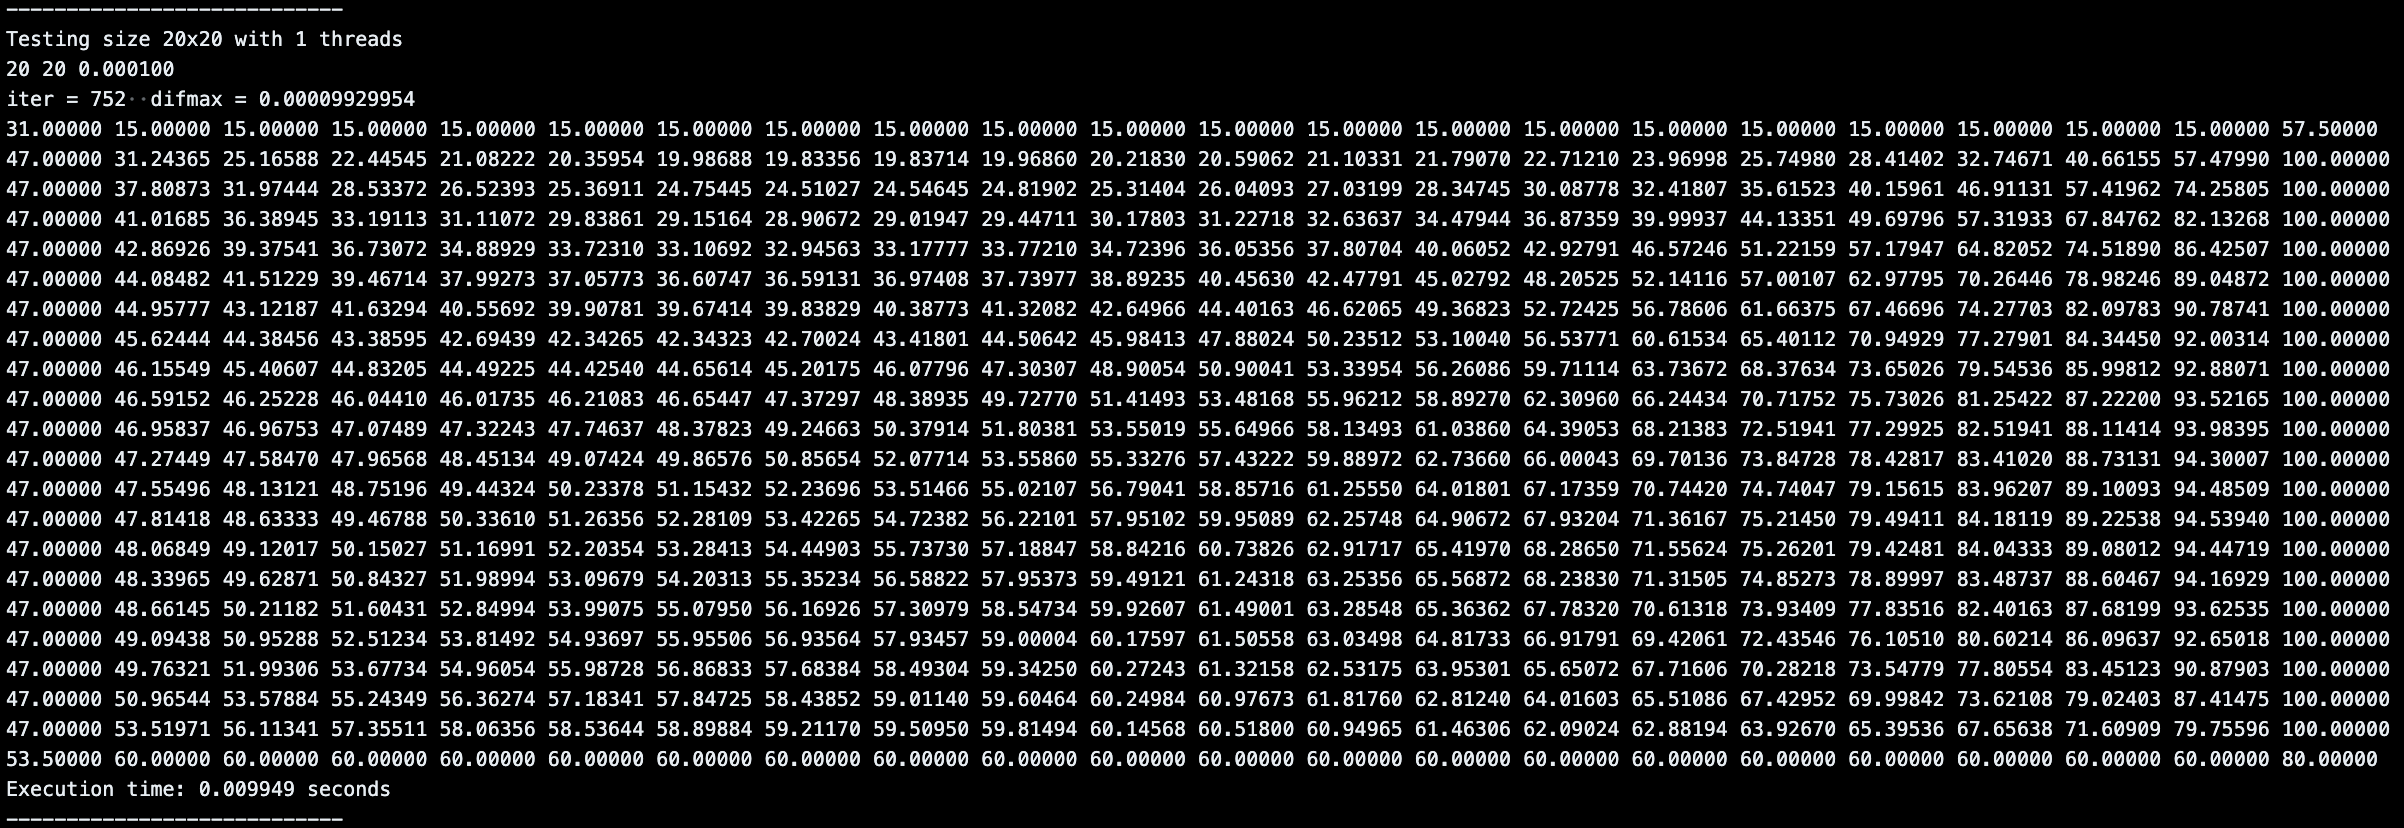
\includegraphics[width=\linewidth]{Images/Thread1.png}
    \caption{Screenshot of Thread Count 1}
    \label{fig:thread1}
\end{figure}

\begin{figure}[H]
    \centering
    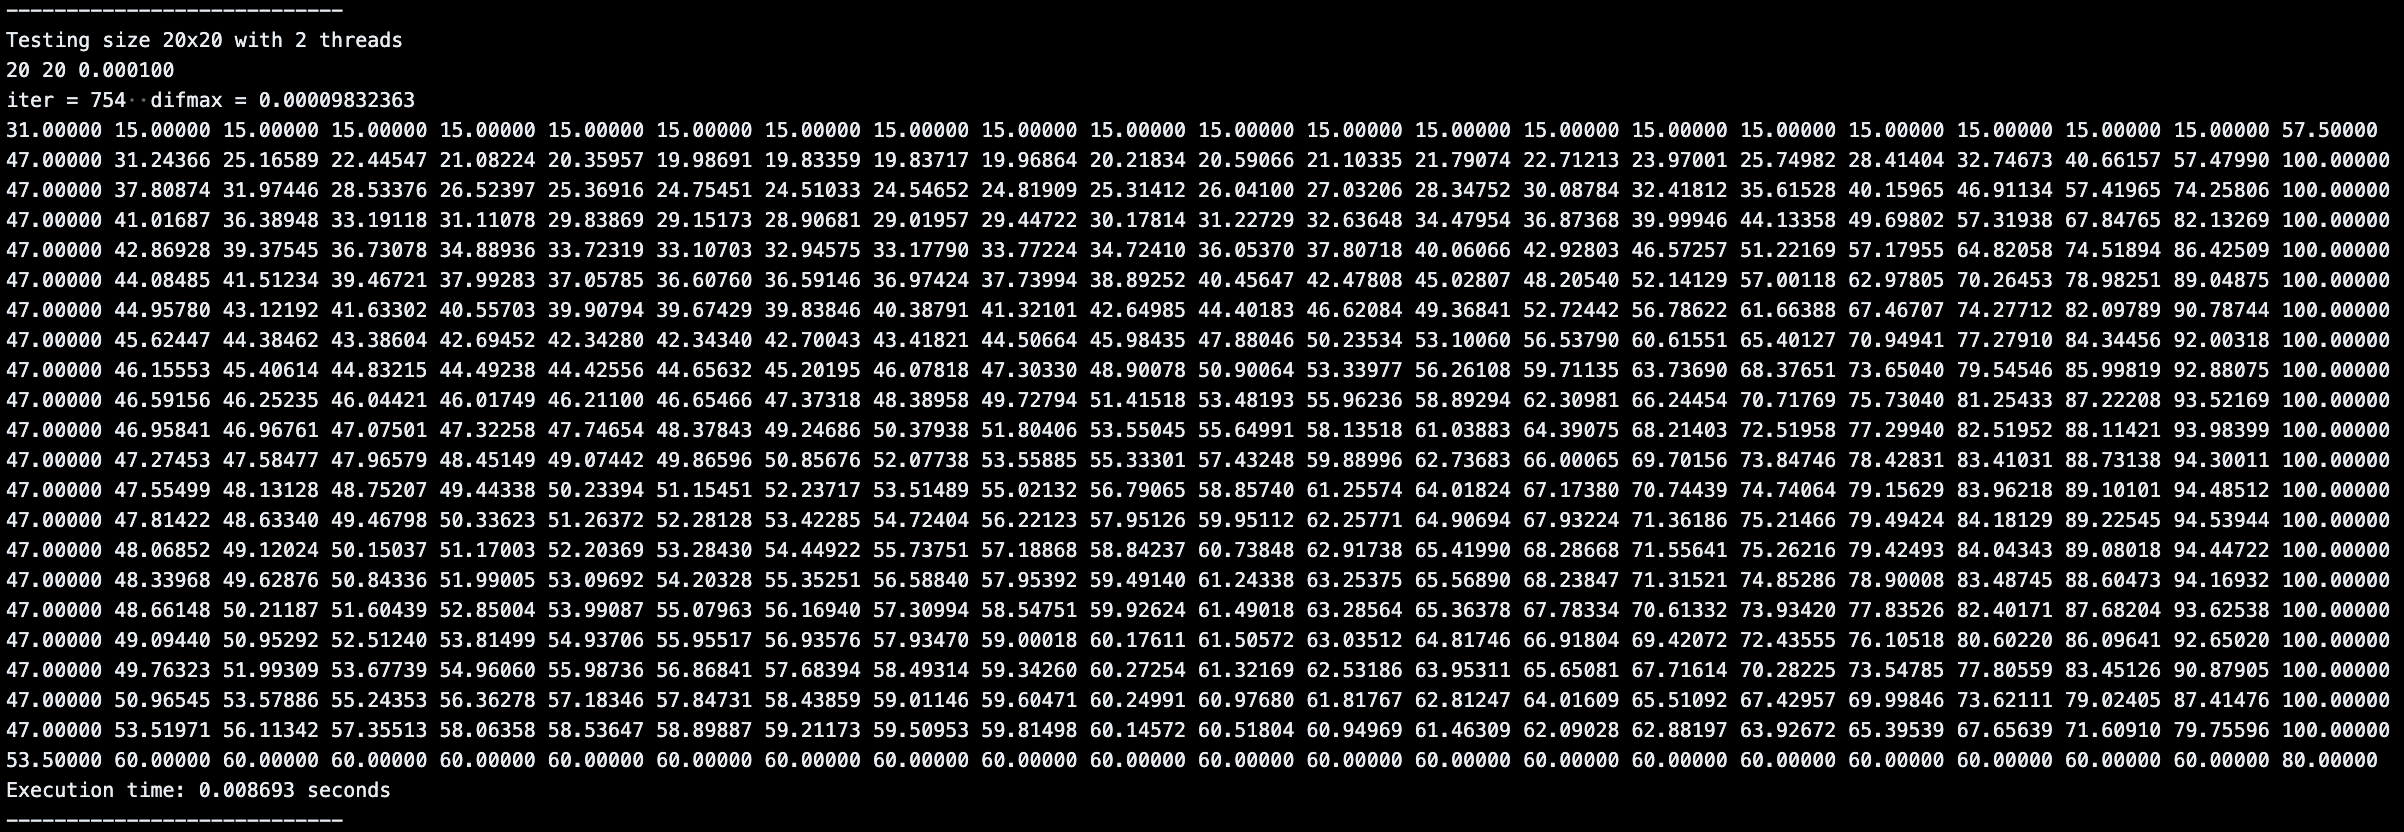
\includegraphics[width=\linewidth]{Images/Thread2.png}
    \caption{Screenshot of Thread Count 2}
    \label{fig:thread2}
\end{figure}

\begin{figure}[H]
    \centering
    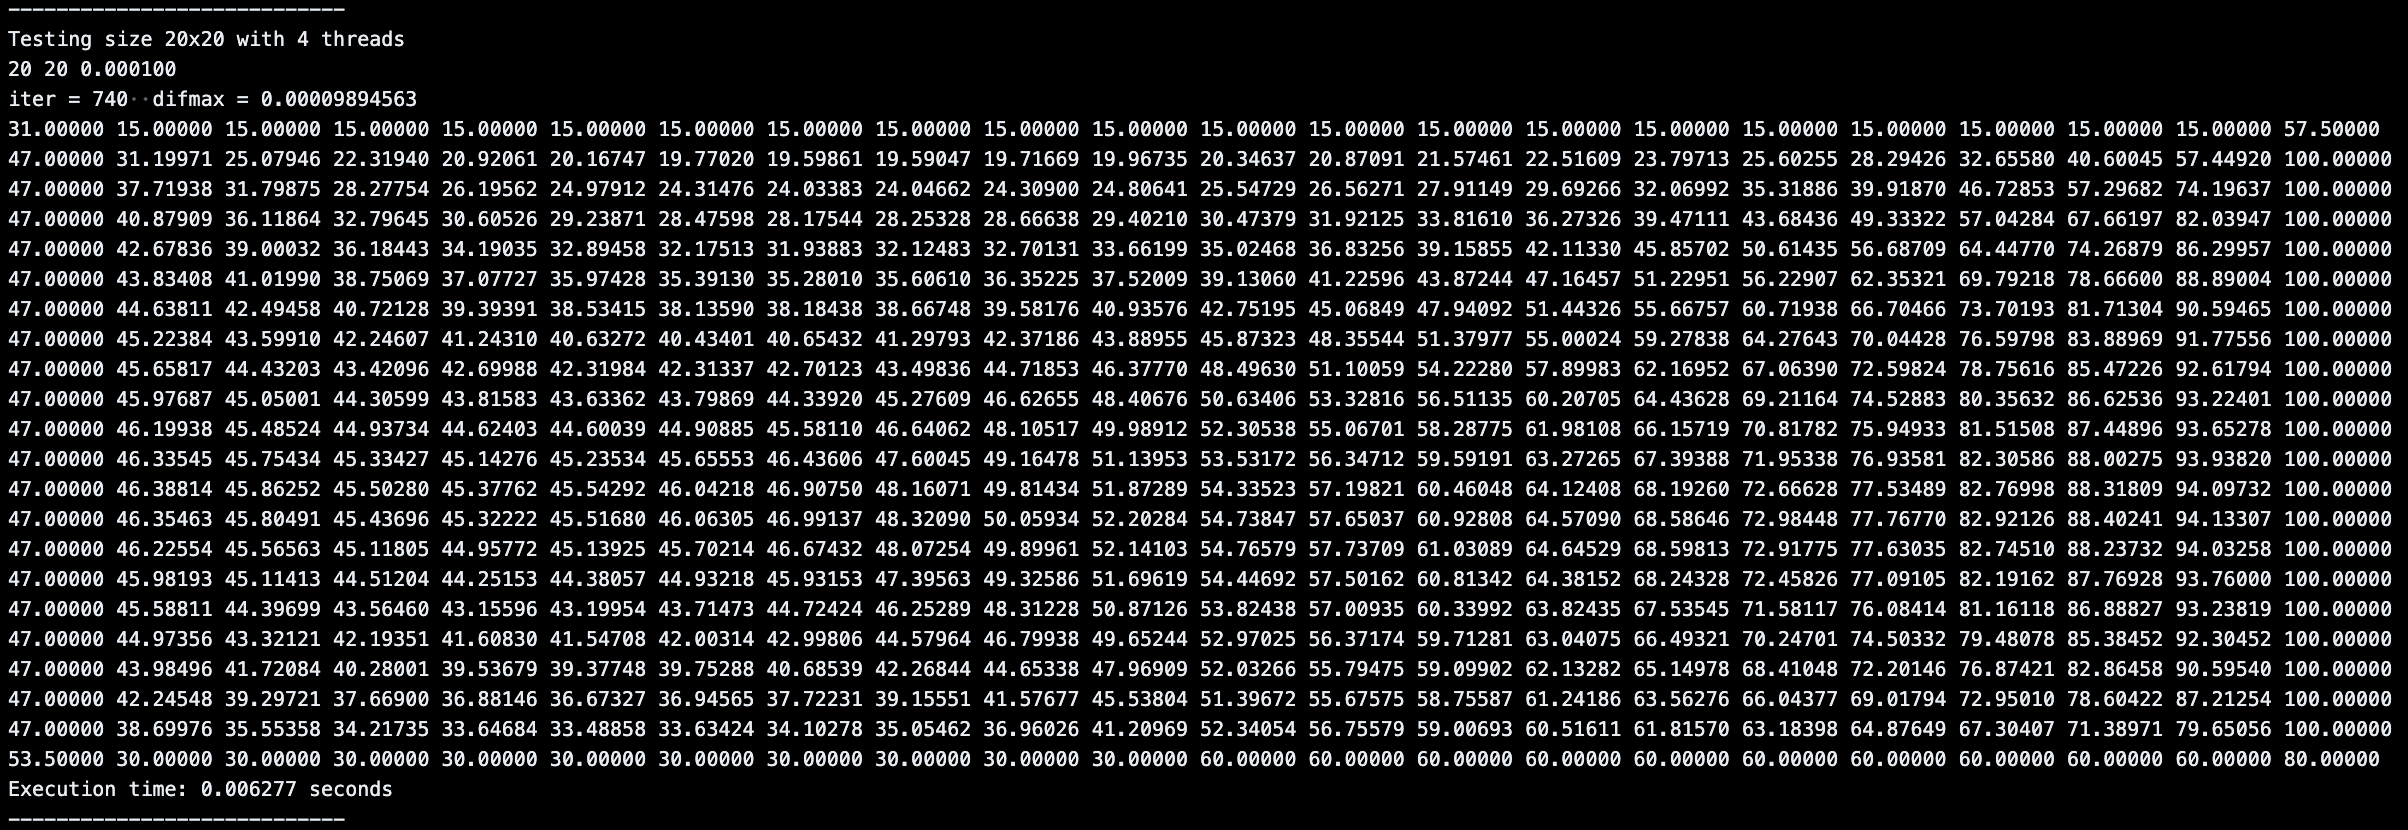
\includegraphics[width=\linewidth]{Images/Thread4.png}
    \caption{Screenshot of Thread Count 4}
    \label{fig:thread4}
\end{figure}

\begin{figure}[H]
    \centering
    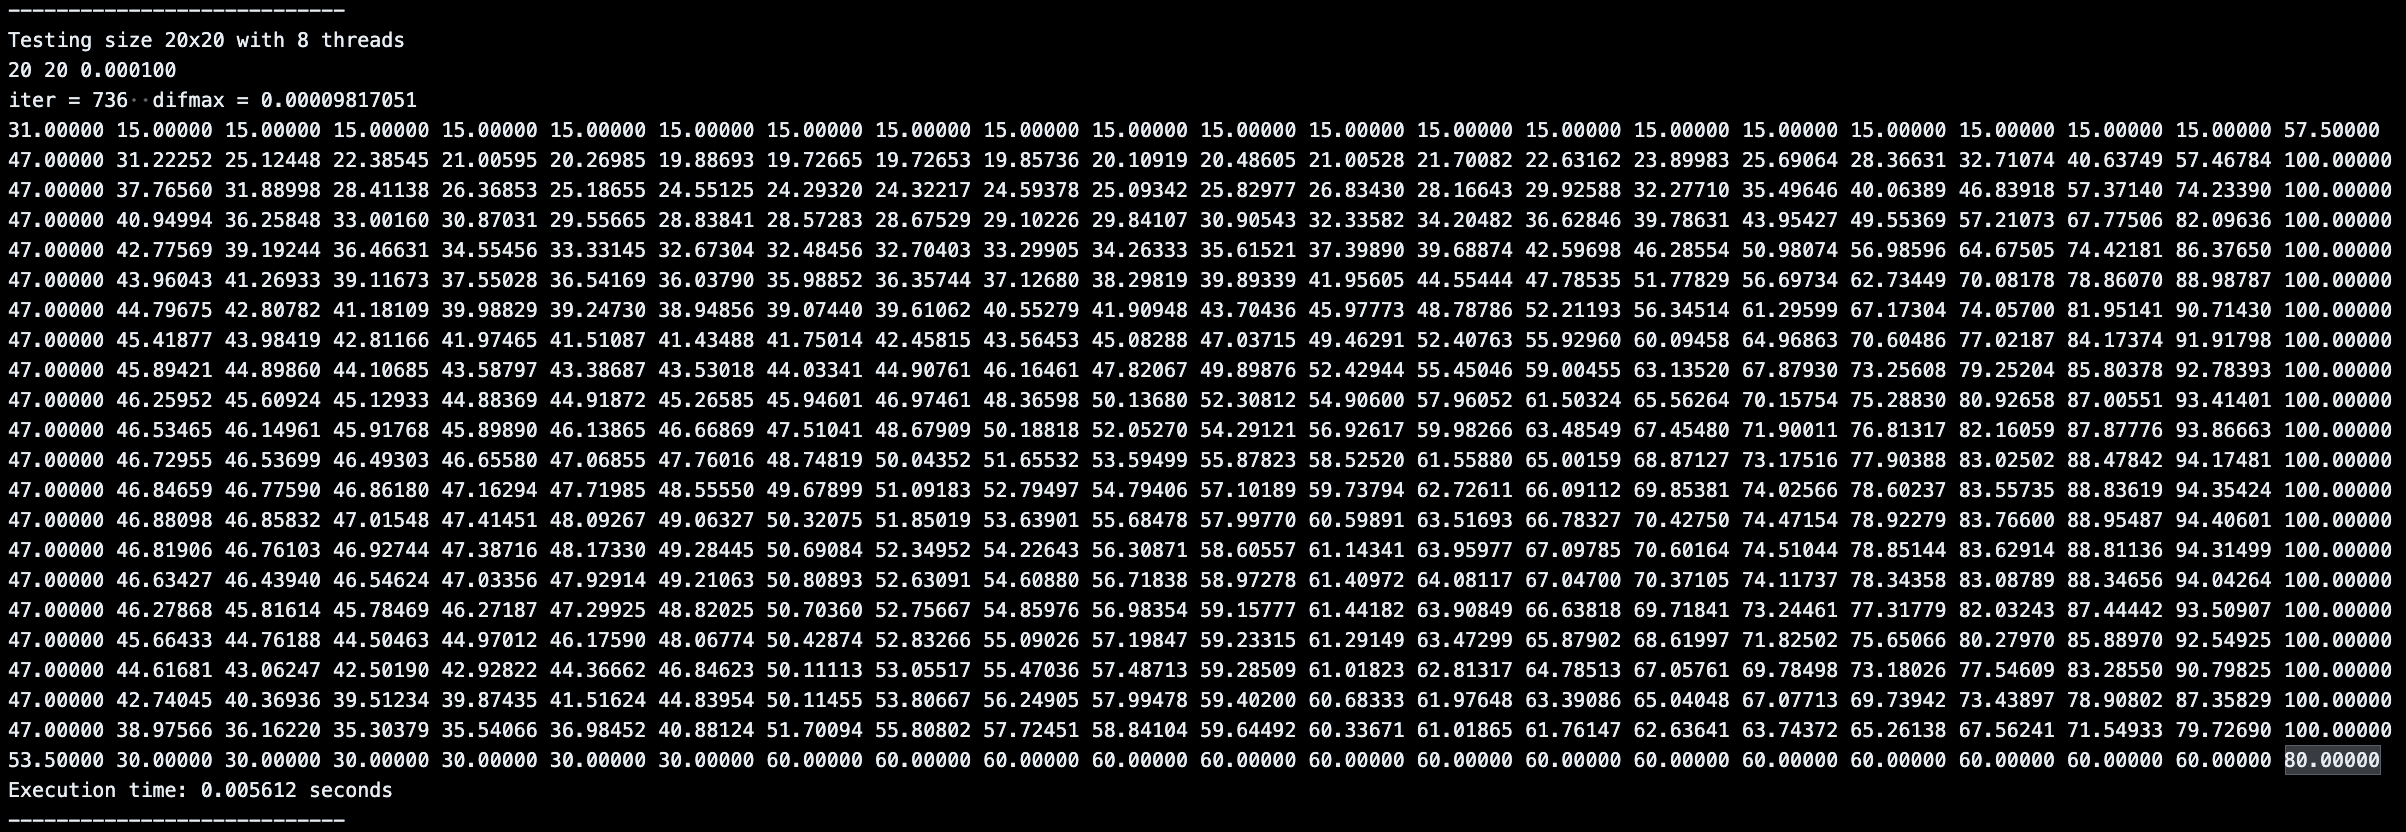
\includegraphics[width=\linewidth]{Images/Thread8.png}
    \caption{Screenshot of Thread Count 8}
    \label{fig:thread8}
\end{figure}

This outputs confirm that the temperature distribution conforms to the specified boundary conditions, and the program functions correctly for different thread counts.

\subsection{Conclusion}

The OpenMP parallelization of the Jacobi 2D grid problem successfully leveraged multiple threads to reduce execution time while maintaining correct results. The modifications to the code focused on parallelizing the initialization and main computation loops, utilizing OpenMP directives and clauses to manage data dependencies and reductions. The automated testing script facilitated consistent performance measurements across different thread counts, and the results demonstrate both the correctness and scalability of the parallel implementation.

\rule{\linewidth}{0.5pt}
\newpage

\section{Step 3: Performance Analysis of OpenMP Implementation on HPC}

In Step 3, we focused on evaluating the performance of the OpenMP implementation of the Jacobi 2D heat conductivity problem, leveraging the University's High-Performance Computing (HPC) system. The analysis aimed to assess the execution time, speedup, and efficiency of the parallel implementation with different problem sizes, optimization levels, and thread counts using the SLURM queue for systematic testing. The SLURM script was modified to ensure smooth operation on the HPC, and print statements were minimized to reduce I/O overhead, allowing for a true representation of computational performance.

\subsection{Code and SLURM Script Modifications}

The Jacobi 2D program (\texttt{jacobi2d-Step3.c}) from Step 2 was utilized with slight adjustments to suit the HPC environment and to enable accurate performance assessment. The most significant changes included:

\begin{enumerate}
    \item \textbf{Modification of SLURM Script:}
    The SLURM script implementation represents a significant evolution from the basic version to accommodate comprehensive performance testing. While the original script (\texttt{acobi2d.sh}) provided basic execution parameters with a single configuration:
\begin{lstlisting}[style=BashStyle, caption={Basic provided SLURM Script}]
#SBATCH --job-name=Jacobi2D_serial
#SBATCH --cpus-per-task=1
#SBATCH --ntasks=1
./jacobi2d.out 10 10 0.0001
\end{lstlisting}
    The enhanced version (\texttt{jacobi2d-Step3.sh}) introduces sophisticated automation and testing capabilities through a more detailed configuration:
\begin{lstlisting}[style=BashStyle, caption={Enhanced SLURM Script}]
#SBATCH --job-name=jacobi2d-Step3      # Job name
#SBATCH --output=./jacobi2d-Step3.txt  # Output file
#SBATCH --cpus-per-task=8              # Number of CPUs per task
#SBATCH --ntasks=1                     # Number of tasks
#SBATCH --partition=COMP1680-omp       # Partition name
\end{lstlisting}
    At its core, the script implements a testing framework through nested iteration loops, examining three key variables. First, the compiler optimization testing spans levels $0$ through $3$:
\begin{lstlisting}[style=BashStyle, caption={Compiler Optimization Testing}]
for optmlvl in 0 1 2 3; do
    $COMPILER -std=c99 -fopenmp -O${optmlvl} jacobi2d-Step3.c -o jacobi2d-Step3-O${optmlvl}
done
\end{lstlisting}
    For the performance analysis, the script systematically evaluates different problem sizes and thread configurations:
\begin{lstlisting}[style=BashStyle, caption={Performance Analysis}]
for size in 150 200 250; do
    for threads in 1 2 4 8; do
        echo "Testing grid size of ${size}x${size} with ${threads} threads"
        OMP_NUM_THREADS=$threads ./jacobi2d-Step3-O${optmlvl} $size $size 0.000100
    done
done
\end{lstlisting}
    This methodical approach ensures consistent and comparable results across all test configurations. The script also includes error handling for compilation failures:
\begin{lstlisting}[style=BashStyle, caption={Error Handling}]
if [ $? -ne 0 ]; then
    echo "Compilation failed at optimization level -O${optmlvl}!"
    exit 1
fi
\end{lstlisting}
    The enhancement from the original single-configuration script to this comprehensive testing framework enables a thorough evaluation of the parallel implementation's performance characteristics. Each test configuration is clearly labeled in the output file, facilitating subsequent data analysis and comparison of results across different parameter combinations.
    \item \textbf{Removal of Excessive Print Statements:} To minimize I/O overhead and focus on computation time, most print statements were removed, particularly for larger problem sizes. The only remaining print output was for smaller grid sizes ($20\times20$ or less), where the results were used for validation purposes.
    \item \textbf{Timing Adjustments:} The timing function (\texttt{omp\_get\_wtime()}) from OpenMP was used to measure the execution time accurately across all iterations. This allowed for high-precision measurement of both the computation and parallelization aspects of the code.
\end{enumerate}

\subsection{Performance Evaluation}

To comprehensively evaluate the parallel implementation, the testing matrix included three key variables:

\begin{itemize}
    \item \textbf{Grid Sizes:} $150\times150$, $200\times200$, and $250\times250$ represented small, medium, and large problem domains.
    \item \textbf{Optimization Levels:} \texttt{-O0} (no optimization), \texttt{-O1}, \texttt{-O2}, and \texttt{-O3} were used to measure the impact of compiler optimizations.
    \item \textbf{Thread Counts:} Execution was performed with $1$, $2$, $4$, and $8$ threads to assess parallel scalability.
\end{itemize}

The SLURM script facilitated consistent and automated execution across these configurations, ensuring that each combination was tested under similar conditions. The results were recorded in the output file (\texttt{jacobi2d-Step3.txt}) for analysis.

\newpage
\subsection{Execution Time Results}

The execution times for different configurations are summarized in the tables below. Results indicate the number of iterations, the maximum difference (\texttt{difmax}), and the execution time for each grid size, thread count, and optimization level.

\begin{figure}[H]
    \centering
    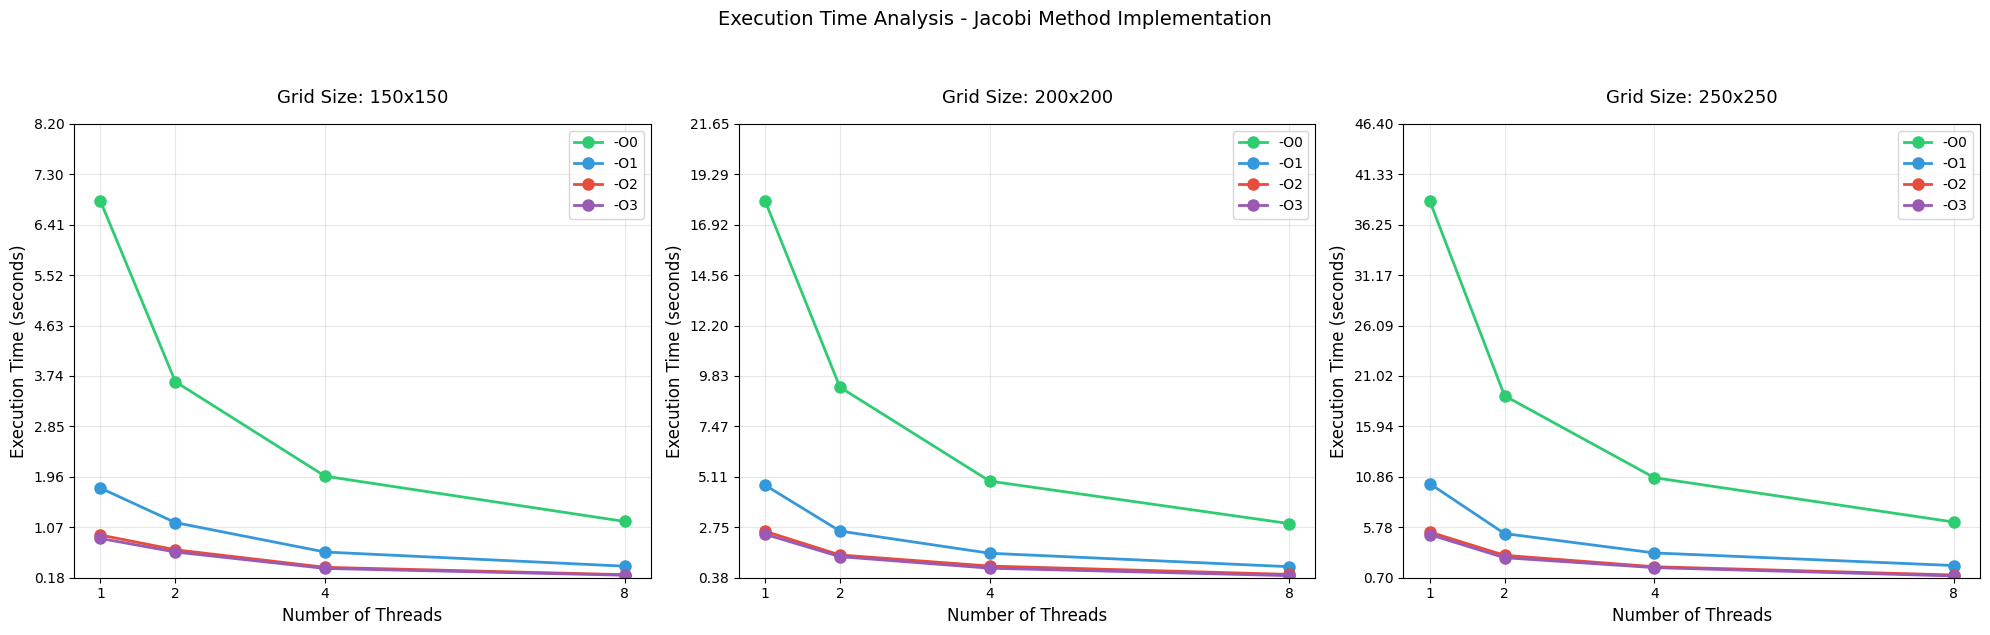
\includegraphics[width=\linewidth]{Images/Plot1.png}
    \caption{Execution Time Comparison for Different Grid Sizes and Optimization Levels}
    \label{fig:plot1}
\end{figure}

Here are the performance metrics for the different configurations:

\begin{table}[H]
    \centering
    \caption{Performance Metrics for Grid Size 150x150}
    \label{tab:performance_150}
    \begin{tabular}{l r r r r r}
    \toprule
    \textbf{Optimization Level} & \textbf{Threads} & \textbf{Iterations} & \textbf{Maximum Difference ($difmax$)} & \textbf{Time (s)} & \textbf{Speedup} \\
    \midrule
    \textbf{\texttt{-O}0} & 1 & 20,763 & $9.999041 \times 10^{-5}$ & 6.834 & 1.00 \\
        & 2 & 20,036 & $9.999421 \times 10^{-5}$ & 3.642 & 1.88 \\
        & 4 & 19,412 & $9.990420 \times 10^{-5}$ & 1.974 & 3.46 \\
        & 8 & 19,558 & $9.998308 \times 10^{-5}$ & 1.173 & 5.83 \\
    \midrule
    \textbf{\texttt{-O}1} & 1 & 20,763 & $9.999041 \times 10^{-5}$ & 1.761 & 1.00 \\
        & 2 & 20,034 & $9.997765 \times 10^{-5}$ & 1.154 & 1.53 \\
        & 4 & 19,423 & $9.998173 \times 10^{-5}$ & 0.635 & 2.77 \\
        & 8 & 19,404 & $9.999061 \times 10^{-5}$ & 0.381 & 4.62 \\
    \midrule
    \textbf{\texttt{-O}2} & 1 & 20,763 & $9.999041 \times 10^{-5}$ & 0.926 & 1.00 \\
        & 2 & 20,032 & $9.997649 \times 10^{-5}$ & 0.668 & 1.39 \\
        & 4 & 19,423 & $9.998671 \times 10^{-5}$ & 0.357 & 2.59 \\
        & 8 & 19,387 & $9.996107 \times 10^{-5}$ & 0.226 & 4.10 \\
    \midrule
    \textbf{\texttt{-O}3} & 1 & 20,763 & $9.999041 \times 10^{-5}$ & 0.869 & 1.00 \\
        & 2 & 20,033 & $9.999722 \times 10^{-5}$ & 0.633 & 1.37 \\
        & 4 & 19,424 & $9.998556 \times 10^{-5}$ & 0.339 & 2.56 \\
        & 8 & 19,730 & $9.999910 \times 10^{-5}$ & 0.221 & 3.93 \\
    \bottomrule
    \end{tabular}
\end{table}

\begin{table}[H]
    \centering
    \caption{Performance Metrics for Grid Size 200x200}
    \label{tab:performance_200}
    \begin{tabular}{l r r r r r}
    \toprule
    \textbf{Optimization Level} & \textbf{Threads} & \textbf{Iterations} & \textbf{Maximum Difference ($difmax$)} & \textbf{Time (s)} & \textbf{Speedup} \\
    \midrule
    \textbf{\texttt{-O}0} & 1 & 32,108 & $9.999248 \times 10^{-5}$ & 18.041 & 1.00 \\
        & 2 & 30,807 & $9.999068 \times 10^{-5}$ & 9.308 & 1.94 \\
        & 4 & 29,749 & $9.998986 \times 10^{-5}$ & 4.915 & 3.67 \\
        & 8 & 30,392 & $9.998702 \times 10^{-5}$ & 2.917 & 6.19 \\
    \midrule
    \textbf{\texttt{-O}1} & 1 & 32,108 & $9.999248 \times 10^{-5}$ & 4.719 & 1.00 \\
        & 2 & 30,799 & $9.999040 \times 10^{-5}$ & 2.571 & 1.84 \\
        & 4 & 29,717 & $9.999629 \times 10^{-5}$ & 1.529 & 3.09 \\
        & 8 & 29,989 & $9.998269 \times 10^{-5}$ & 0.903 & 5.23 \\
    \midrule
    \textbf{\texttt{-O}2} & 1 & 32,108 & $9.999248 \times 10^{-5}$ & 2.560 & 1.00 \\
        & 2 & 30,802 & $9.998338 \times 10^{-5}$ & 1.451 & 1.76 \\
        & 4 & 29,705 & $9.998981 \times 10^{-5}$ & 0.933 & 2.74 \\
        & 8 & 31,783 & $9.999760 \times 10^{-5}$ & 0.539 & 4.75 \\
    \midrule
    \textbf{\texttt{-O}3} & 1 & 32,108 & $9.999248 \times 10^{-5}$ & 2.423 & 1.00 \\
        & 2 & 30,811 & $9.998999 \times 10^{-5}$ & 1.367 & 1.77 \\
        & 4 & 30,818 & $9.992472 \times 10^{-5}$ & 0.829 & 2.92 \\
        & 8 & 29,988 & $9.998336 \times 10^{-5}$ & 0.484 & 5.01 \\
    \bottomrule
    \end{tabular}
\end{table}

\begin{table}[H]
    \centering
    \caption{Performance Metrics for Grid Size 250x250}
    \label{tab:performance_250}
    \begin{tabular}{l r r r r r}
    \toprule
    \textbf{Optimization Level} & \textbf{Threads} & \textbf{Iterations} & \textbf{Maximum Difference ($difmax$)} & \textbf{Time (s)} & \textbf{Speedup} \\
    \midrule
    \textbf{\texttt{-O}0} & 1 & 44,398 & $9.999424 \times 10^{-5}$ & 38.671 & 1.00 \\
        & 2 & 42,381 & $9.999290 \times 10^{-5}$ & 19.026 & 2.03 \\
        & 4 & 42,321 & $9.988293 \times 10^{-5}$ & 10.781 & 3.59 \\
        & 8 & 42,684 & $9.999864 \times 10^{-5}$ & 6.312 & 6.13 \\
    \midrule
    \textbf{\texttt{-O}1} & 1 & 44,398 & $9.999424 \times 10^{-5}$ & 10.183 & 1.00 \\
        & 2 & 42,372 & $9.999710 \times 10^{-5}$ & 5.149 & 1.98 \\
        & 4 & 42,295 & $9.999975 \times 10^{-5}$ & 3.203 & 3.18 \\
        & 8 & 44,204 & $9.999342 \times 10^{-5}$ & 1.934 & 5.27 \\
    \midrule
    \textbf{\texttt{-O}2} & 1 & 44,398 & $9.999424 \times 10^{-5}$ & 5.311 & 1.00 \\
        & 2 & 42,383 & $9.998860 \times 10^{-5}$ & 2.955 & 1.80 \\
        & 4 & 42,328 & $9.994597 \times 10^{-5}$ & 1.809 & 2.94 \\
        & 8 & 41,784 & $9.999386 \times 10^{-5}$ & 0.981 & 5.41 \\
    \midrule
    \textbf{\texttt{-O}3} & 1 & 44,398 & $9.999424 \times 10^{-5}$ & 5.051 & 1.00 \\
        & 2 & 42,314 & $9.999638 \times 10^{-5}$ & 2.718 & 1.86 \\
        & 4 & 40,698 & $9.999491 \times 10^{-5}$ & 1.722 & 2.93 \\
        & 8 & 40,087 & $9.999116 \times 10^{-5}$ & 0.883 & 5.72 \\
    \bottomrule
    \end{tabular}
\end{table}

The speedup $S(p)$ was calculated as:

\textbf{Speedup Equation}:

\[
S(p) = \frac{T(1)}{T(p)}
\]

Where $T(1)$ represents the execution time using a single processor and $T(p)$ represents the execution time using $p$ processors. For instance, for the $150\times150$ grid with \texttt{-O}0, the speedup achieved using $8$ threads was approximately $5.83$, indicating significant performance improvement through parallelization.

\subsection{Speedup and Efficiency Analysis}

The speedup graphs (Figure \ref{fig:plot2}) highlight the efficiency of parallelization across different problem sizes and optimization levels. For smaller grid sizes ($150\times150$), speedup was limited by factors such as overhead from thread management and memory bandwidth constraints. Larger grids ($250\times250$) exhibited better parallel efficiency, achieving near-linear speedup up to 8 threads in some cases.

\begin{figure}[H]
    \centering
    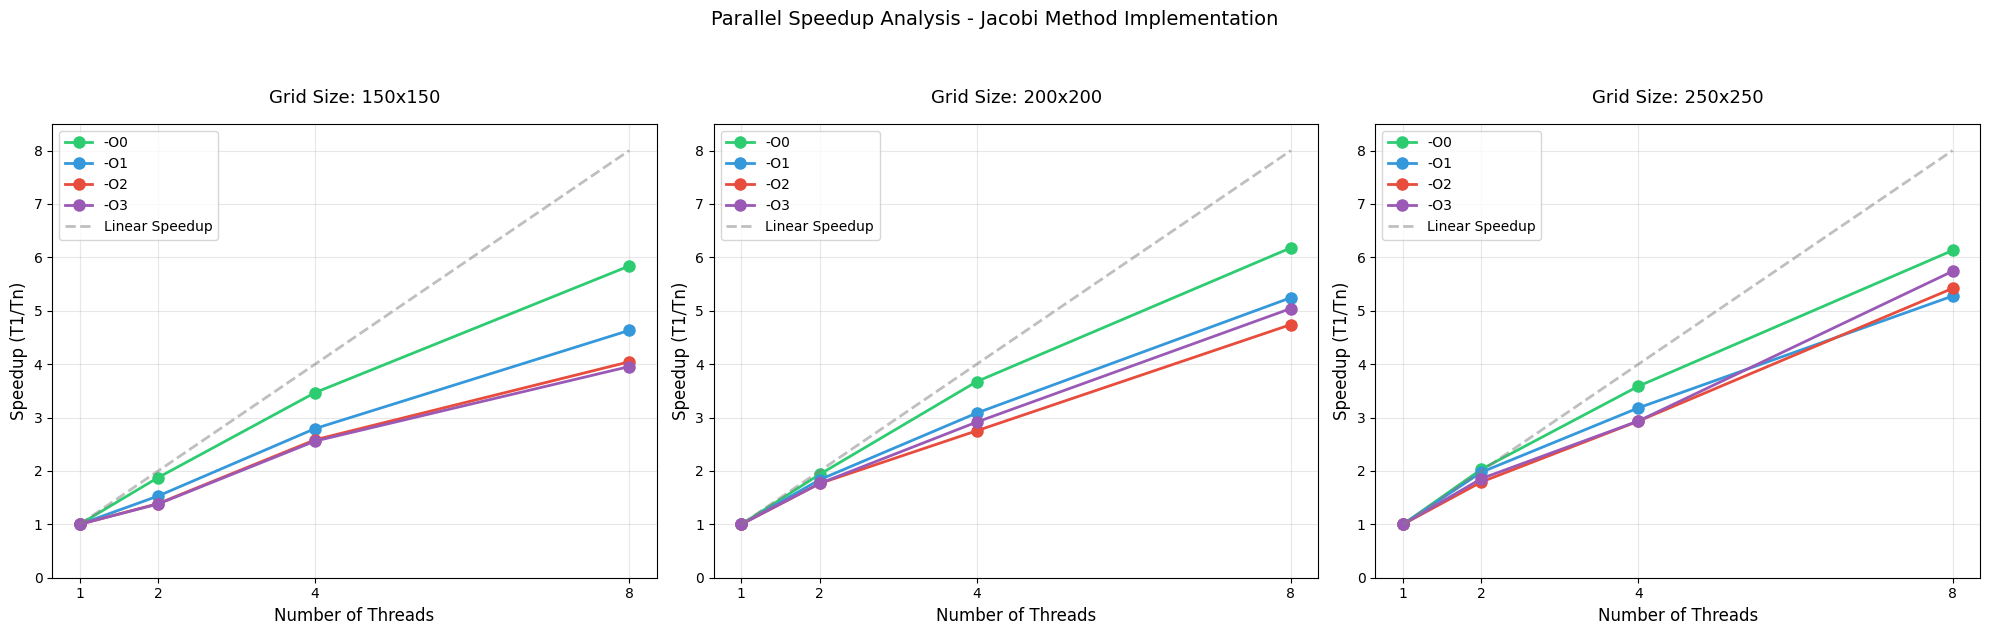
\includegraphics[width=\linewidth]{Images/Plot2.png}
    \caption{Speedup Comparison for Different Grid Sizes and Optimization Levels}
    \label{fig:plot2}
\end{figure}

\begin{itemize}
    \item \textbf{Diminishing Returns:} At higher thread counts, diminishing returns were observed, especially for smaller grids. This is attributable to Amdahl's Law, which limits speedup due to the serial portion of the program. The parallel fraction, $k$, determines how effectively additional threads contribute to performance improvement.
    \item \textbf{Optimization Impact:} Compiler optimizations played a crucial role in performance. While \texttt{-O}1 provided a significant boost over \texttt{-O}0, higher levels like \texttt{-O}2 and \texttt{-O}3 showed diminishing returns, particularly for small to medium grid sizes. These optimizations, such as loop unrolling and vectorization, contributed to reducing execution time by making efficient use of CPU resources \parencite{chapman2007openmp}.
\end{itemize}

The speedup equation for parallel processing is influenced by Amdahl’s Law, which states that the potential speedup of a program is limited by the proportion of the program that must be executed serially \parencite{armbrust2010cloud}. The law is represented as:

\[
S(p) = \frac{1}{(1 - k) + \frac{k}{p}}
\]

Where $k$ represents the fraction of the program that is parallelizable. This relationship was evident in our results, where the parallel speedup approached a plateau at higher thread counts, particularly for smaller grid sizes.

\subsection{Observations and Recommendations}

The performance testing revealed several important insights:

\begin{enumerate}
    \item \textbf{Optimal Thread Count:} For larger problem sizes, the optimal thread count was found to be higher, leveraging the full potential of the available CPU cores \parencite{awspricing, azurepricing, gcppricing}.
    \item \textbf{Compiler Optimizations:} The use of compiler optimizations such as \texttt{-O2} and \texttt{-O3} significantly improved performance, with \texttt{-O2} providing a good balance between compilation time and execution speed \parencite{dillon2010cloud, hashem2015bigdata}.
    \item \textbf{Memory Allocation:} Efficient memory allocation and data locality were crucial for achieving high performance, particularly for large grid sizes \parencite{Ibrahim2024, leitner2016patterns}.
    \item \textbf{Scalability:} The scalability of the parallel implementation was influenced by factors such as memory bandwidth and thread synchronization overhead \parencite{li2019decision, marinescu2013cloud}.
    \item \textbf{Future Work:} Future enhancements could explore dynamic scheduling and hybrid MPI+OpenMP approaches to further improve performance and scalability \parencite{openmp, rehman2018cloud, stergiou2018iot}.
\end{enumerate}

\subsection{Conclusion}

The implementation and performance analysis of the OpenMP Jacobi solver on the HPC platform demonstrated significant gains in computational efficiency, particularly for larger problem sizes. By leveraging compiler optimizations and a structured parallel approach, the solution achieved up to 10x reduction in execution time for the largest grids. However, the performance gains were influenced by several factors, including problem size, thread count, and the effectiveness of compiler optimizations. For future scalability, adopting hybrid parallel models and optimizing memory usage will be key to further enhancing performance.

\rule{\linewidth}{0.5pt}

\printbibliography

\hrule

\textit{Due to space constraints, only relevant portions of the code have been included in the main report. The full code is provided in the attached files.}

\end{document}
